%%%%%%%%%%%%%%%%%%%%%%%%%%%%%%%%%%%%%%%%%%%%%%%
%
% Template per Elaborato di Laurea
% DISI - Dipartimento di Ingegneria e Scienza dell’Informazione
%
% update 2015-09-10
%
% Per la generazione corretta del 
% pdflatex nome_file.tex
% bibtex nome_file.aux
% pdflatex nome_file.tex
% pdflatex nome_file.tex
%
%%%%%%%%%%%%%%%%%%%%%%%%%%%%%%%%%%%%%%%%%%%%%%%

% formato FRONTE RETRO
\documentclass[epsfig, a4paper, 11pt, titlepage, twoside, openany]{book}
\usepackage{epsfig}
\usepackage{plain}
\usepackage{setspace}
\usepackage{array}
\usepackage{afterpage}
\usepackage[paperheight=29.7cm, paperwidth=21cm, outer=1.5cm, inner=2.5cm, top=2cm, bottom=2cm]{geometry} % per definizione layout
\usepackage{titlesec} % per formato custom dei titoli dei capitoli

%%%%%%%%%%%%%%
% supporto lettere accentate
%
%\usepackage[latin1]{inputenc} % per Windows;
%\usepackage[utf8x]{inputenc} % per Linux (richiede il pacchetto unicode);
\usepackage[applemac]{inputenc} % per Mac.

\singlespacing

\usepackage[english]{babel}
\usepackage{chngcntr}
\counterwithout{footnote}{chapter}

\begin{document}

  % nessuna numerazione
  \pagenumbering{gobble} 
  \pagestyle{plain}

\thispagestyle{empty}

\vspace{1.2 cm}

\begin{center}
  \begin{figure}[h!]
    \centerline{
\psfig{file=marchio_unitrento_colore_it_v2.eps,width=0.66\textwidth}}
  \end{figure}
  
  \vspace{2.2 cm}
  
  \LARGE{Department of Information Engineering and Computer Science\\}
  
  \vspace{1.2 cm}
  \Large{Bachelor's Degree in\\
    Information and Communications Engineering
  }
  
  \vspace{2.2 cm}
  \Large\textsc{Final Dissertation\\}
  \vspace{1.2 cm}
  % \Huge\textsc{Crowd density estimation system\\based on Wi-Fi probe request frames\\}
  \Huge\textsc{A system for estimating\\crowd density based on\\Wi-Fi probe request frames\\}
  
  \vspace{2.2 cm}
  \begin{tabular*}{\textwidth}{ c @{\extracolsep{\fill}} c }
  \Large{Supervisors} & \Large{Student}\\
  \Large{Fabrizio Granelli} & \Large{Samuel Bortolin}\\
  \Large{Daniele Miorandi} & \\
  \end{tabular*}
  
  \vspace{2.2 cm}
  \Large{Academic year 2019/2020}
  
\end{center}

  \cleardoublepage
 
%%%%%%%%%%%%%%%%%%%%%%%%%%%%%%%%%%%%%%%%%%%%%%%%%%%%%%%%%%%%%%%%%%%%%%%%%%
%%%%%%%%%%%%%%%%%%%%%%%%%%%%%%%%%%%%%%%%%%%%%%%%%%%%%%%%%%%%%%%%%%%%%%%%%%
%% Nota
%%%%%%%%%%%%%%%%%%%%%%%%%%%%%%%%%%%%%%%%%%%%%%%%%%%%%%%%%%%%%%%%%%%%%%%%%%
%% Sezione Ringraziamenti opzionale
%%%%%%%%%%%%%%%%%%%%%%%%%%%%%%%%%%%%%%%%%%%%%%%%%%%%%%%%%%%%%%%%%%%%%%%%%%
%%%%%%%%%%%%%%%%%%%%%%%%%%%%%%%%%%%%%%%%%%%%%%%%%%%%%%%%%%%%%%%%%%%%%%%%%%
  \thispagestyle{empty}

\begin{center}
  {\bf \Huge Acknowledgments}
\end{center}

\vspace{4cm}


\emph{
  \dots{ thanks to my family, my girlfriend, my supervisors and all the U-Hopper Team }\dots
}

  \afterpage{\null\thispagestyle{empty}\clearpage}
  \pagestyle{plain} % nessuna intestazione e pie pagina con numero al centro

  
  % inizio numerazione pagine in numeri arabi
  \mainmatter

%%%%%%%%%%%%%%%%%%%%%%%%%%%%%%%%%%%%%%%%%%%%%%%%%%%%%%%%%%%%%%%%%%%%%%%%%%
%%%%%%%%%%%%%%%%%%%%%%%%%%%%%%%%%%%%%%%%%%%%%%%%%%%%%%%%%%%%%%%%%%%%%%%%%%
%% Nota
%%%%%%%%%%%%%%%%%%%%%%%%%%%%%%%%%%%%%%%%%%%%%%%%%%%%%%%%%%%%%%%%%%%%%%%%%%
%% Si ricorda che il numero massimo di facciate e' 30.
%% Nel conteggio delle facciate sono incluse 
%%   indice
%%   sommario
%%   capitoli
%% Dal conteggio delle facciate sono escluse
%%   frontespizio
%%   ringraziamenti
%%   allegati    
%%%%%%%%%%%%%%%%%%%%%%%%%%%%%%%%%%%%%%%%%%%%%%%%%%%%%%%%%%%%%%%%%%%%%%%%%%
%%%%%%%%%%%%%%%%%%%%%%%%%%%%%%%%%%%%%%%%%%%%%%%%%%%%%%%%%%%%%%%%%%%%%%%%%%

    % indice
    \tableofcontents
    \afterpage{\null\thispagestyle{empty}\clearpage}
          
    % gruppo per definizone di successione capitoli senza interruzione di pagina
    \begingroup
      % nessuna interruzione di pagina tra capitoli
      % ridefinizione dei comandi di clear page
      %\renewcommand{\cleardoublepage}{} 
      %\renewcommand{\clearpage}{} 
      % redefinizione del formato del titolo del capitolo
      % da formato
      %   Capitolo X
      %   Titolo capitolo
      % a formato
      %   X   Titolo capitolo
      
      \titleformat{\chapter}
        {\normalfont\Huge\bfseries}{\thechapter}{1em}{}
        
      \titlespacing*{\chapter}{0pt}{0.59in}{0.02in}
      \titlespacing*{\section}{0pt}{0.20in}{0.02in}
      \titlespacing*{\subsection}{0pt}{0.10in}{0.02in}
      
      % sommario
      \chapter*{Abstract} % senza numerazione
\label{abstract}

\addcontentsline{toc}{chapter}{Abstract} % da aggiungere comunque all'indice
\vspace{0.4 cm} 

Being able to estimate the number of people in your business, especially in this moment of crisis caused by the spread of COVID-19, represents a great opportunity for companies that have to deal with physical customers, both to offer their customers optimal service both to optimize your resources. The system developed, once adapted to the particular service offered by the company, allows you to optimally manage the demand for your service by providing an accurate estimate of customers at all times. From this information, the management of departments of the activity under analysis can understand when it is necessary to increase the amount of service provided and when it is possible to reduce saving important resources.

Employing your employees to manually count the people requesting the service at all times, think of the case of a bus or a supermarket, would be very frustrating for the employees but above all expensive. After an in-depth study of the current state of the art and of the different technologies developed for this purpose, it was decided that the optimal solution to obtain this information is to exploit the Wi-Fi signals coming from the devices of its customers to estimate their actual number.

This thesis project was carried out at U-Hopper during my external internship. The work I did was to improve an existing system and be able to make it more versatile and robust, providing real-time data transmission and allowing the system to be adapted to multiple use cases.

I worked a lot on the data collection part, implementing a code on a Raspberry Pi that allowed to detect particular frames for the connection management from all Wi-Fi packets, i.e. the probe request frames from which it was possible to extract information useful for processing, ensuring the privacy of its customers by anonymizing the MAC address.

Much of the processing that is done on the data to get people estimates has been designed to run on a server. By developing a code for cleaning the collected data I was able to detect the number of devices present at all times in the vicinity of the Raspberry Pi. Subsequently, through a part of machine learning, properly calibrated with the ground truth that I collected manually, i.e. the real number of people, I was able to estimate the number of people present.

In order to connect these two parts I used MQTT communication protocol, versatile and scalable, and I developed the whole part for data transmission with an MQTT client on the Raspberry Pi and another one on the server. Also on the server, in our case the U-Hopper one was used, an MQTT broker was executed to forward the data to the receiver client and a database for the storage of the data received by the Raspberry Pi on which it is then possible to carry out the analysis.

The functioning of this system was initially tested at home, due to the restrictions imposed on people on their personal mobility, and subsequently validated in a place of social interest with a certain dynamism, a Cafe, once the restrictions ceased. The results obtained at the end of processing, adequately compared with manually-collected ground truth, are in line with initial expectations. In conclusion, the system provides a good estimate of the number of people present with a mean absolute error of less than two people. This was possible mainly thanks to a careful calibration of the machine learning model, which was initially developed by U-Hopper's colleagues for another project, which I perfected in order to conduct my analyzes and obtain the desired results.

      \afterpage{\null\thispagestyle{empty}\clearpage}

%%%%%%%%%%%%%%%%%%%%%%%%%%%%%%%%%%%%%%%%%%%%%%%%%%%%%%%%%%%%%%%%%%%%%%%%%%
%%%%%%%%%%%%%%%%%%%%%%%%%%%%%%%%%%%%%%%%%%%%%%%%%%%%%%%%%%%%%%%%%%%%%%%%%%
%% Nota
%%%%%%%%%%%%%%%%%%%%%%%%%%%%%%%%%%%%%%%%%%%%%%%%%%%%%%%%%%%%%%%%%%%%%%%%%%
%% Sommario e' un breve riassunto del lavoro svolto dove si descrive 
%% l’obiettivo, l’oggetto della tesi, le metodologie e 
%% le tecniche usate, i dati elaborati e la spiegazione delle conclusioni 
%% alle quali siete arrivati.
%% Il sommario dell’elaborato consiste al massimo di 3 pagine e deve contenere le seguenti informazioni: 
%%   contesto e motivazioni
%%   breve riassunto del problema affrontato
%%   tecniche utilizzate e/o sviluppate
%%   risultati raggiunti, sottolineando il contributo personale del laureando/a
%%%%%%%%%%%%%%%%%%%%%%%%%%%%%%%%%%%%%%%%%%%%%%%%%%%%%%%%%%%%%%%%%%%%%%%%%%
%%%%%%%%%%%%%%%%%%%%%%%%%%%%%%%%%%%%%%%%%%%%%%%%%%%%%%%%%%%%%%%%%%%%%%%%%%      
      
      %%%%%%%%%%%%%%%%%%%%%%%%%%%%%%%%
      % lista dei capitoli
      %
      % \input oppure \include
      %
      \chapter{Introduction}
\label{cha:intro}
\vspace{0.4 cm} 

In this chapter, a brief introduction of the internship and the project done at U-Hopper\footnote{ website: \url{https://www.u-hopper.com/} } is presented.
I chose to do my internship at U-Hopper, a deep-tech company that develops big data analytics, business intelligence and artificial intelligence solutions, in the heart of the Dolomites.
U-Hopper operates at the intersection of three technological axes: internet of things, big data and artificial intelligence, with the aim of providing analytics to companies and enabling personalized services for their users.
U-Hopper brings together research and development skills and proven experience in the design and development of high quality ICT solutions.


\section{Problem statement}
\label{sec:problem}
\vspace{0.2 cm} 

In managing a company that provides services to physical customers, the most important aspect is how to manage the flow of customers to guarantee them optimal service. Overcrowding and long waiting times are serious problems caused by poor demand management. These problems spoil the service experience of the users and especially during this pandemic period due to COVID-19, it is important to avoid generating crowds and queues to avoid new contagions. The repetition of these events leads to the loss of customers and therefore to the loss of revenue for the company. This fact is increasingly relevant in this period of crisis with very low liquidity.

Offering an efficient and fast service is the key to increasing the number of customers in their own business. The solution is not to use all the available resources to try to meet these requirements, as excessive use of these leads to an increase in costs without leading to an increase in revenues.
Of course, in order to calibrate the correct amount of service to offer, it would be necessary to know the demand. In particular it is necessary to know every time how many people require the service. Having this information is not trivial as it is highly variable over time and depends on several factors.

The purpose of this thesis is to create a system capable of providing useful information to a company's organizational departments to manage its resources more effectively and efficiently. In particular, the proposed system will provide estimates of the number of customers in real-time through the use of machine learning techniques.
From this information, it will be possible to understand how the demand is distributed over time and what the peak hours are. This will clarify in which time slots it is necessary to increase the capacity of the service in order to be able to provide it to a greater number of people. In a dual way, this information is also useful for understanding when there is less demand and it is possible to reduce the capacity of the service, with the aim of saving resources.

The idea can also be extended to provide the same crowding data to its customers. With this data, they can plan better when to use the service offered, avoiding being in crowded situations or situations that require long waiting times.


\section{Approach to the problem} 
\label{sec:approach}
\vspace{0.2 cm} 

After analyzing the current state of the art and the different methods used in literature to count/estimate people in different fields of application and the different implementations, the approach chosen to solve this problem is to use the Wi-Fi probe request frames.
In the 802.11 standards, there are the management frames to manage the connection between access points and devices. The most important for us is the probe request frame, a particular frame that a device sends to check if there is a known access point in the area that sends a probe response frame to allow the connection.

Why is this important? From this type of frame, it is possible to extract the MAC address of the device (usually randomized if not connected), the RSSI (unstable, but it provides an indication of the distance), the SSID (network for which the device is probing), the sequence counter and the time (when the probe is detected).

The Research Statement is: Is it possible to continuously estimate the density of the crowd in a place of interest based on the Wi-Fi probe request frames?

The Thesis Objectives are:
\begin{itemize}
  \item Capture and analysis of Wi-Fi probe request frames.
  \item Data extraction, transmission and storage.
  \item Analysis of Wi-Fi probe request frames patterns.
  \item Provide an estimation of the number of customers.
\end{itemize}

Why Wi-Fi solution?
High diffusion of Wi-Fi devices, low-cost implementation (use of a Raspberry Pi for data collection), real-time data transmission (using MQTT protocol), user privacy ensured (anonymization of MAC addresses).

What was made?
I designed and developed a system for this problem that could work in several contexts.
Sniffing the probe request frames using a Raspberry Pi running a Python program that uses the Scapy library. Then, sending batches to a server using MQTT and analyzing the collected data through a regression that has been optimized with machine learning.
The system was tested in a Cafe and I collected 4 weeks of data and manually-annotated ground truth to validate and evaluate the functioning.


\section{Outline} 
\label{sec:outline}
\vspace{0.2 cm} 

In chapter~\ref{cha:soa} the state of the art is analyzed.
In chapter~\ref{cha:system} the methodology and the choices in the system design are presented.
Chapter~\ref{cha:implementation}  presents how the system is implemented.
In chapter~\ref{cha:evaluation} the proposed system is validated and the results are evaluated.
In the end, chapter~\ref{cha:conclusions} reports the conclusions and suggests some ideas for future work.

      \afterpage{\null\thispagestyle{empty}\clearpage}
      \chapter{State of the Art}
\label{cha:soa}
\vspace{0.5 cm} 

Literature review \dots


\vspace{0.5 cm} 
\section{Crowd analysis}
\label{sec:crowd}
\vspace{0.5 cm} 

Analyze the crowd \dots


\vspace{0.5 cm} 
\section{People counting methods}
\label{sec:count}
\vspace{0.5 cm} 

What are the methods for count the people \dots


\vspace{0.5 cm} 
\subsection{People estimation on buses}
\label{sec:bus}
\vspace{0.5 cm}


\vspace{0.5 cm} 
\subsection{Why probe requests?}
\label{sec:probe}
\vspace{0.5 cm}

Here there are two interesting articles
\cite{mikkelsen2016public}
\cite{mehmood2019occupancy}

% viene tenuto l'ordine per cognome nelle citazioni in automatico

Something else \dots
\cite{nishide2019filter}

      \afterpage{\null\thispagestyle{empty}\clearpage}
      \chapter{System Design}
\label{cha:system}
\vspace{0.4 cm} 

In this chapter, the methodology and the choices in the system design are presented. Starting by describing the components of the system with their functionalities (i.e. the blocks in the system architecture) and then explaining the working logic of the developed system. After this chapter, it will be clear which are the main parts of this system and how they cooperate to achieve the project goal.


\section{System architecture}
\label{sec:sysarc}
\vspace{0.2 cm} 

In a place of interest, there are people/users with their devices that are sending Wi-Fi packets, if they have the Wi-Fi device turned on. The purpose of our system is to exploit these packets to infer the number of people present. The system architecture of the developed system is shown in figure~\ref{fig:architecture}.
This is a distributed architecture, in fact, there are three main components on different platforms that cooperate over a communication network in order to achieve this goal.

\begin{figure}[h]
\centering 
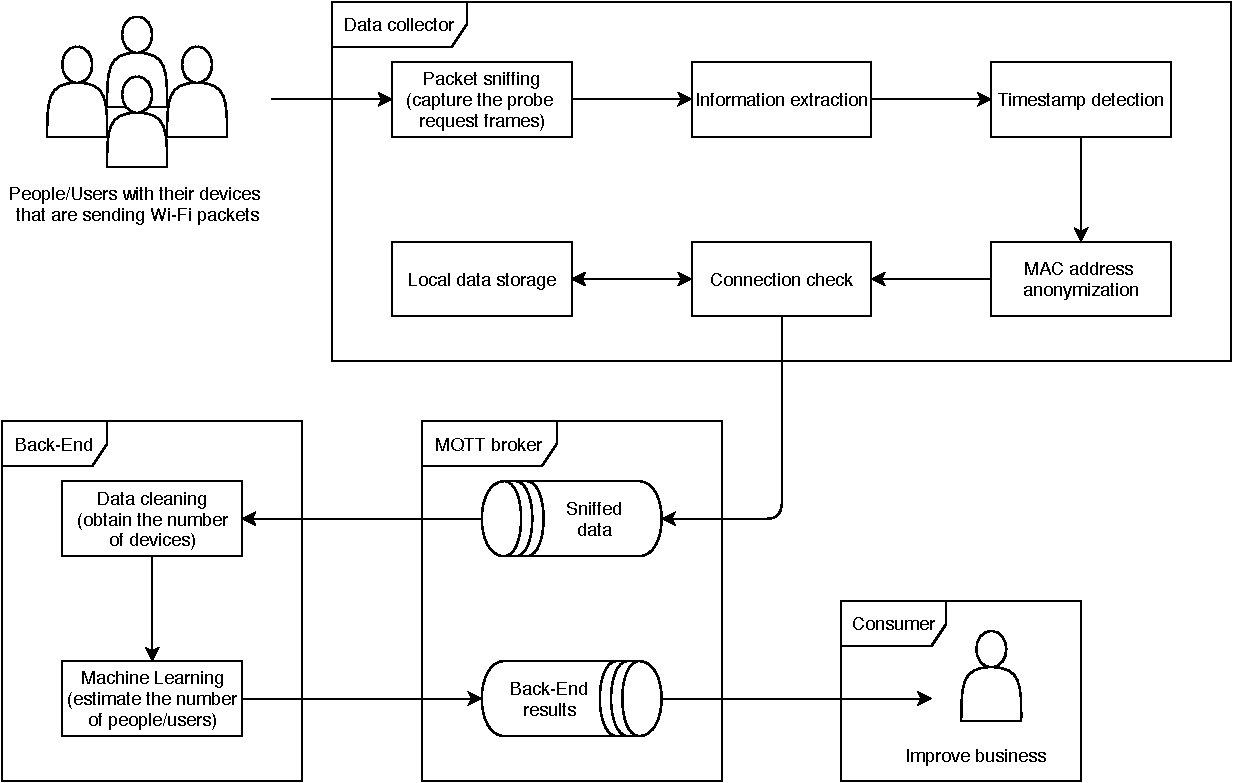
\includegraphics[width=0.9\textwidth]{images/architecture} 
\caption{Architecture of the proposed system.}
\label{fig:architecture}
\end{figure}

The first block of the system is a data collector which is located in the place of interest. It performs a preprocessing of the data (distributed work) with its functionalities: sniffing of Wi-Fi packets, capture the probe request frames; extract the useful information from these; detect the current timestamp; anonymize the MAC address using a hash function (no more privacy issues); check the internet connection; if there is no connection, save the data in the local storage; if there is a connection, publish the collected data to the dedicated queue.

The system uses the MQTT protocol for data forwarding, using an MQTT broker situated on a server, it must have a static IP address to be accessible, the broker has two dedicated queues: one for the collected data, published by the data collector and received by the subscribed receiver in the Back-End part, and the other one for the Back-End results published by the Back-End part after the analysis and received by the subscribed consumer.

The Back-End part is situated on a server. Initially, it deals with collected data receiving and storing in a database. Then, it deals with data cleaning: RSSI thresholding, remove random encounters (and randomized MAC addresses are removed with this), make a blacklist to remove the ever-present devices or devices revealed too many times during the day and therefore get the number of devices present in the place of interest. Finally, it deals with data analysis using machine learning: fit the degree and the coefficients of the polynomial approximation using the trend and the seasonality of the number of devices detected to get the number of people present and publication of the results to the dedicated queue.

At the end of this processing, there is the consumer who receives the results of the Back-End, i.e. the number of people in the place of interest, and could use this information to improve his business.

This architecture is scalable, it could admit many sensors physically distributed in different environments for data collection, to provide a practical example some use cases are shown in figure~\ref{fig:excases}. It is important to locate them properly in the environments to cover all the areas of interest. All sensors publish data to the same MQTT broker and then all data is forwarded to the same Back-End. Cleaning and analysis will be performed according to the data source, each sensor will publish data in its own reserved queue and will be analyzed adequately to the characteristics of the use case for which it was used. In the end, results are sent to the respective consumer through an appropriate queue.

\begin{figure}[h]
\centering 
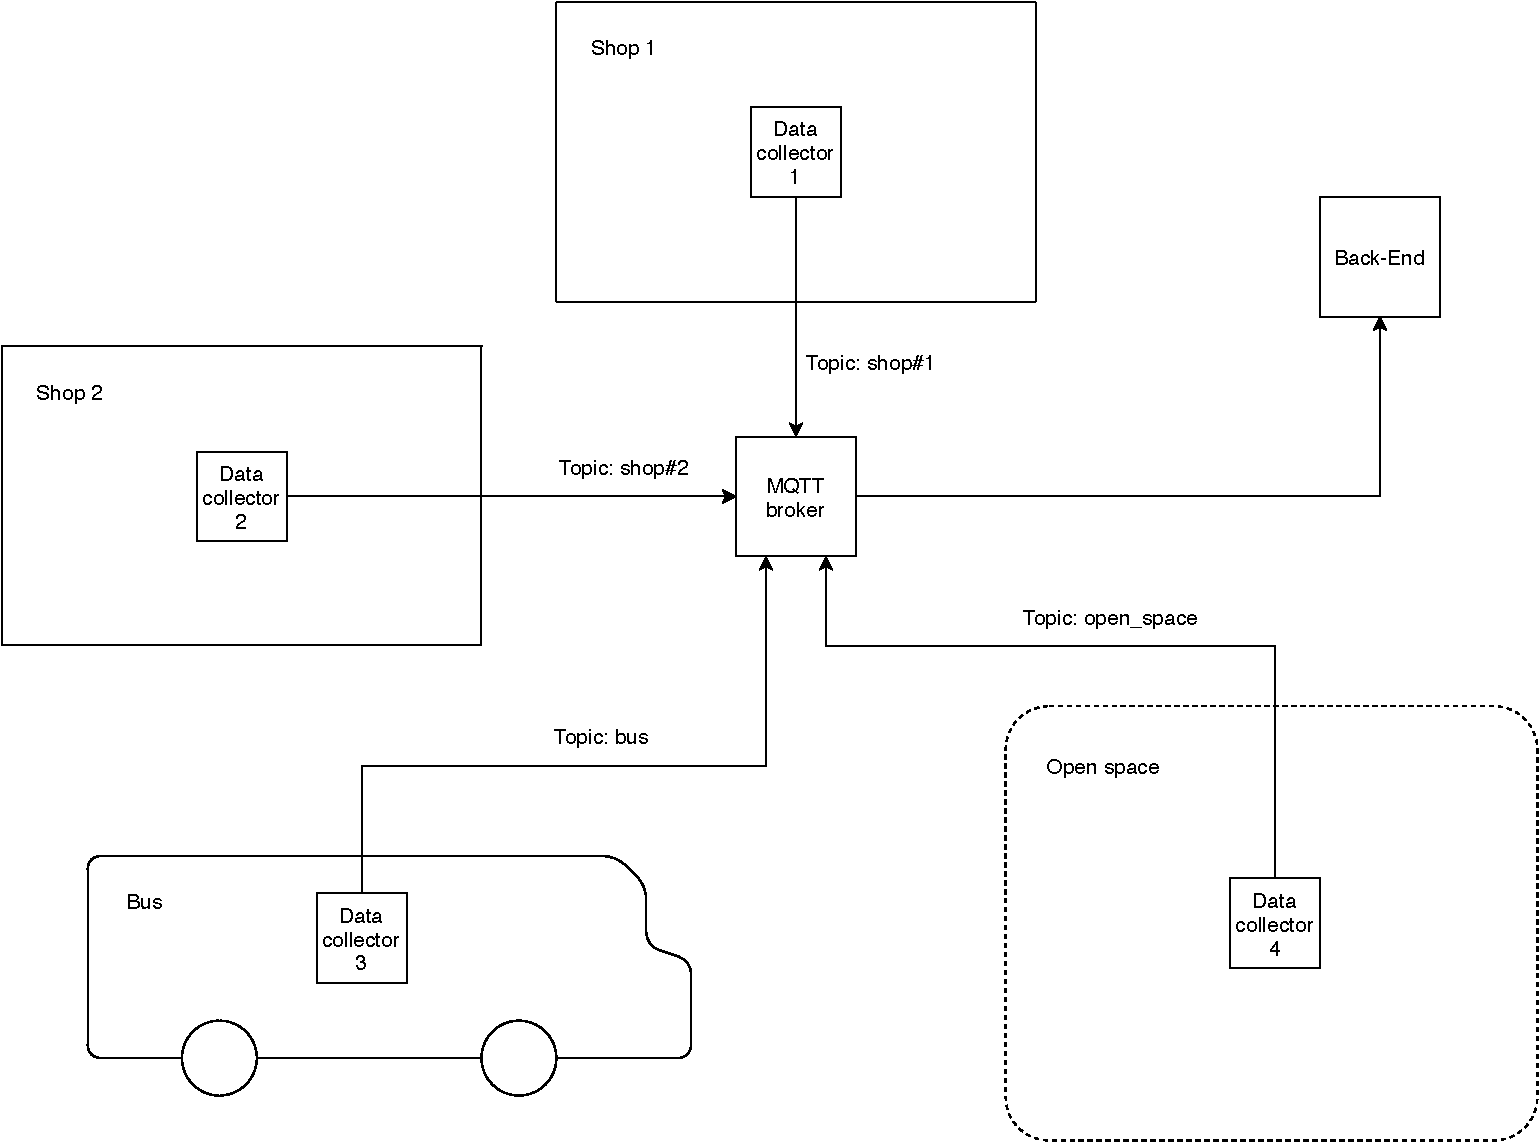
\includegraphics[width=0.9\textwidth]{images/excases} 
\caption{Presentation of a possible implementation with different use cases.}
\label{fig:excases}
\end{figure}


\section{Data collection}
\label{sec:collection}
\vspace{0.2 cm} 

The main block I worked on is the data collector. I developed the logic behind this block, with particular attention in the research of the connection and in the management of the data collected.

The flowchart representing the data collector logic is shown in figure~\ref{fig:flowcollect}. When the data collector is turned on, the system searches for the connected Wi-Fi dongle and puts it in monitor mode to perform the packet sniffing. Initially, a packet counter is set = 0 and the actual timestamp is saved. When a packet is received, it checks if it is a probe request frame and if it is not, it is thrown away.
When a probe request frame is captured, the following information are extracted: RSSI, SSID (Service Set Identifier), MAC address, sequence counter. The timestamp when the packet was revealed together with the other information are saved and the packet counter increases by one.

\begin{figure}[h!]
\centering 
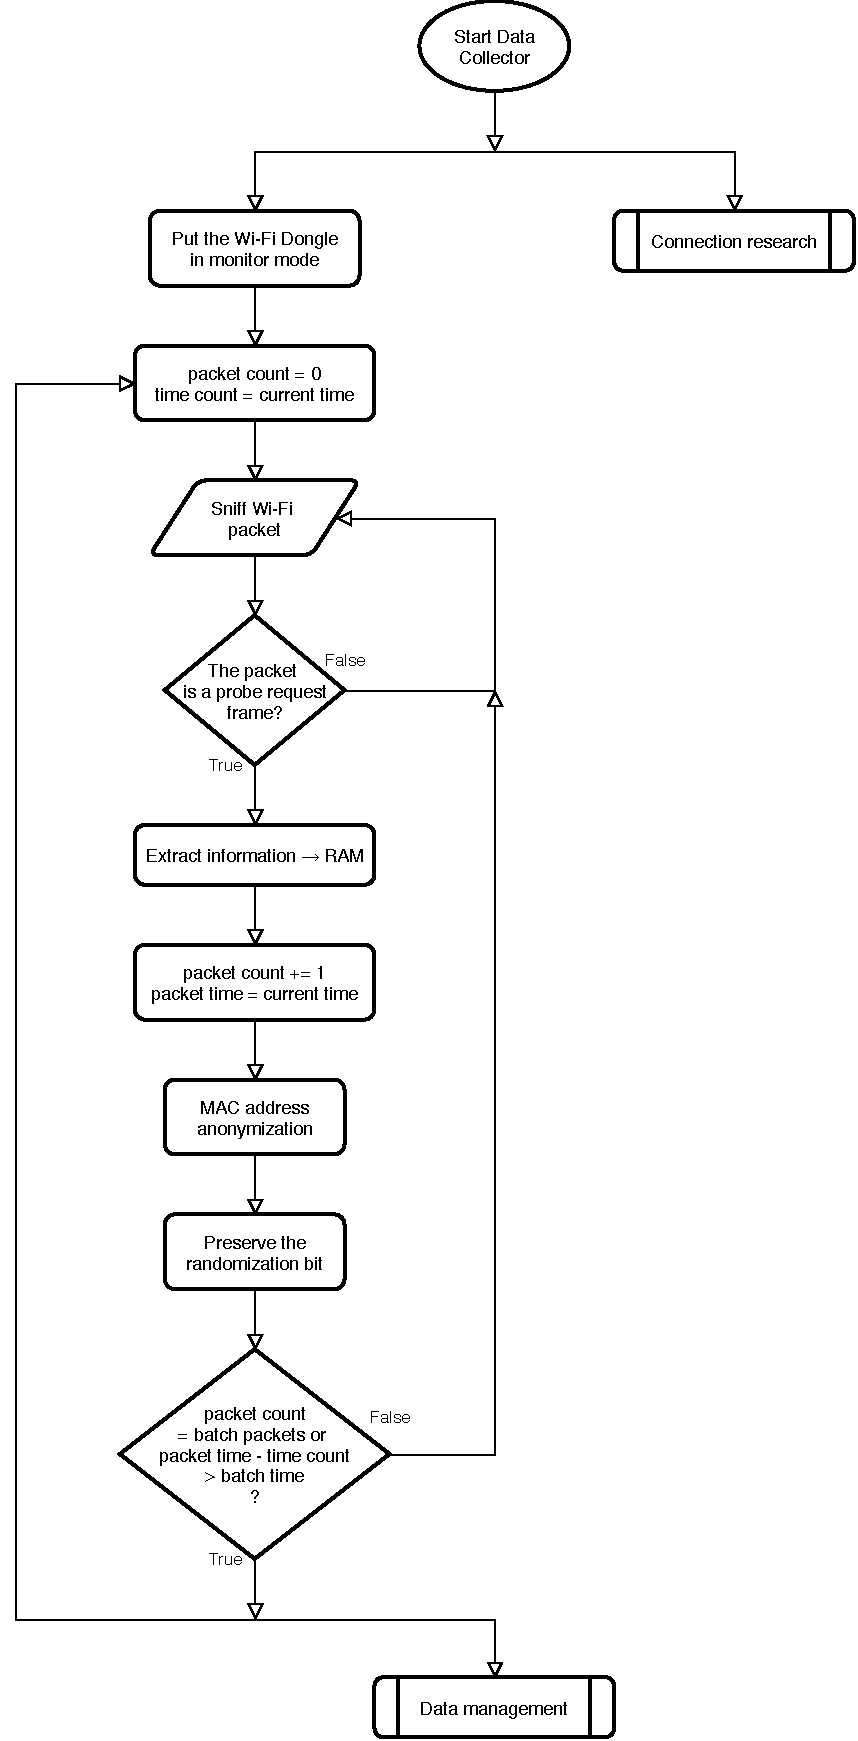
\includegraphics[width=0.45\textwidth]{images/flowcollect} 
\caption{Flowchart representing the data collector logic.}
\label{fig:flowcollect}
\end{figure}

% \begin{wrapfloat}{figure}{I}{0pt} 
% 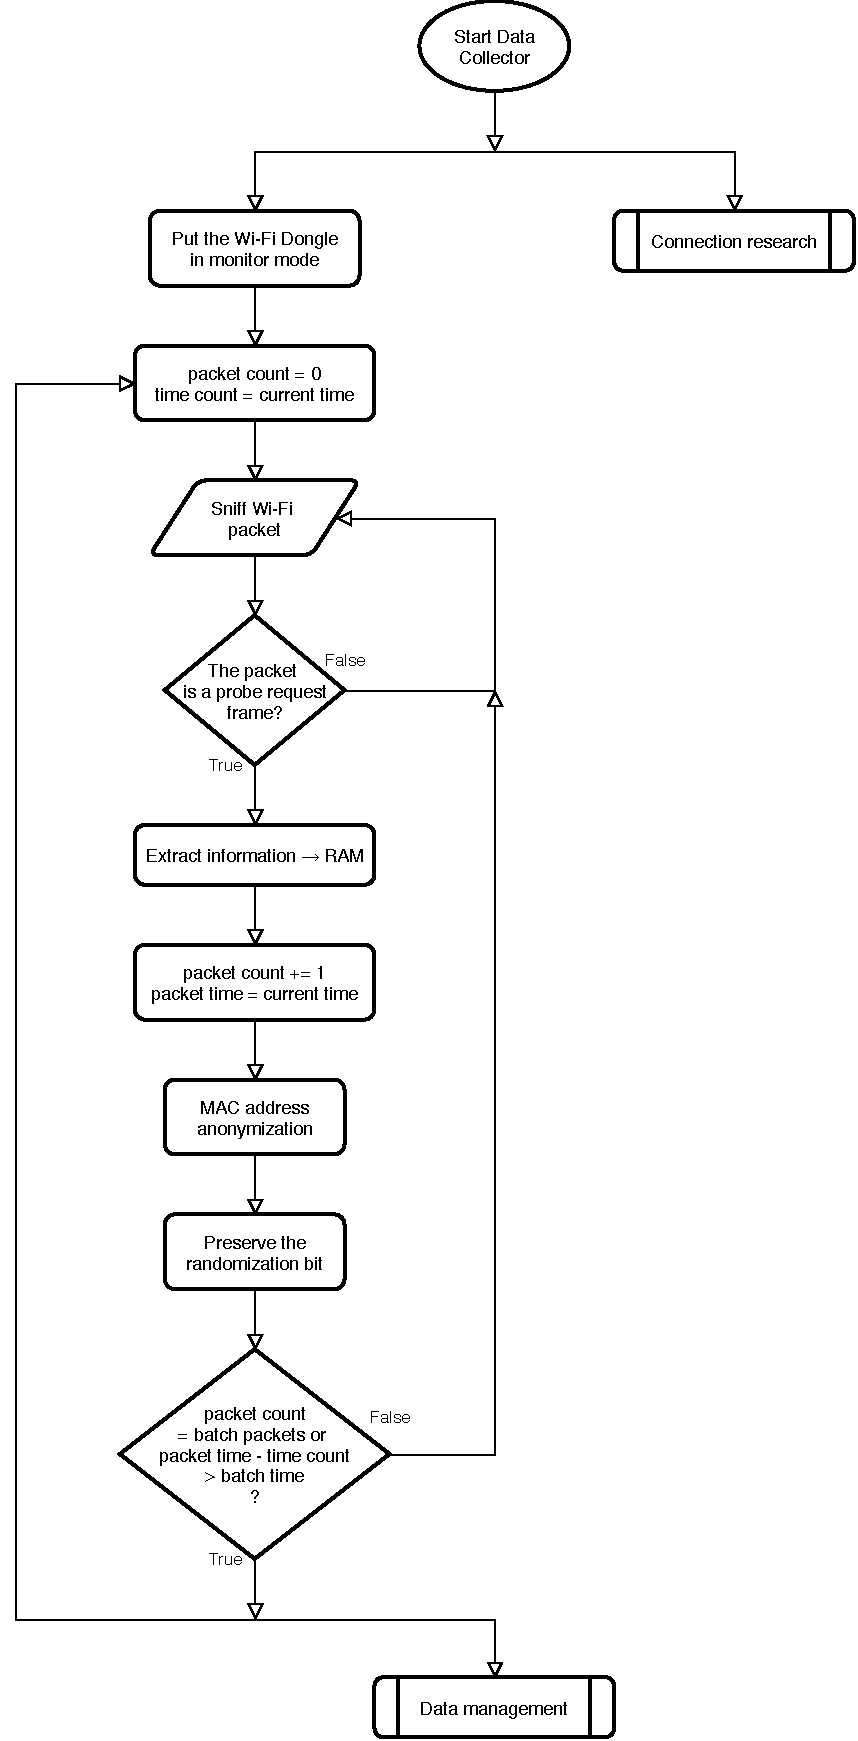
\includegraphics[width=0.5\textwidth]{images/flowcollect}
% \caption{Flowchart representing the data collector logic.}
% \label{fig:flowcollect}
% \end{wrapfloat}

Among the information that can be extracted from the MAC address before performing the anonymization there are the OUI (Organizationally Unique Identifier), from which the manufacturer of the device can be identified, and the local bit, the 7\textsuperscript{th} bit of the MAC address, from which it can be seen whether the MAC address is randomized or not.

After extracting the information, there is the anonymization of the MAC address to preserve the privacy of the users and comply with the GDPR. This is made only for the MAC addresses that are not randomized, i.e. the real MAC addresses of the devices present. Anonymization is performed at this point in the architecture because then there are no more privacy problems, this work does not have to be done from the Back-End and for reasons of data security in case of a data breach during transmission.
This process consists of hashing the MAC address using the BLAKE2 cryptographic hash function\footnote{ website: \url{https://blake2.net/} } (BLAKE3 is faster but still under development). BLAKE2 is faster than MD5, SHA-1, SHA-2 and SHA-3, and provides security superior to SHA-2 and similar to that of SHA-3. BLAKE2 supports keying and salting, and can output digests from 1 up to 32 or 64 bytes depending on the version. This hash function is the ideal for changing hash results every 24 hours or predefined time, simply modifying the key or adding a different value of salt. This is made for privacy reasons and to avoid tracing the MAC address although it is not the real one but always the same after hashing.
If the anonymization changes the state of the local bit, the previous state is forced/imposed to preserve this information on randomization, which can be used in the cleaning phase.

Once the pre-processing of the data is completed, we decided to process the collected data in batches and therefore there are to check 2 batch criteria, based on a maximum number of packets and a maximum time since the last batch transmission. These parameters have to be set according to the use case/case study, once one of these is reached it is possible to decide what to do with this data by running the data management flowchart, shown in figure~\ref{fig:flowdata}.

\begin{figure}[h]
\centering 
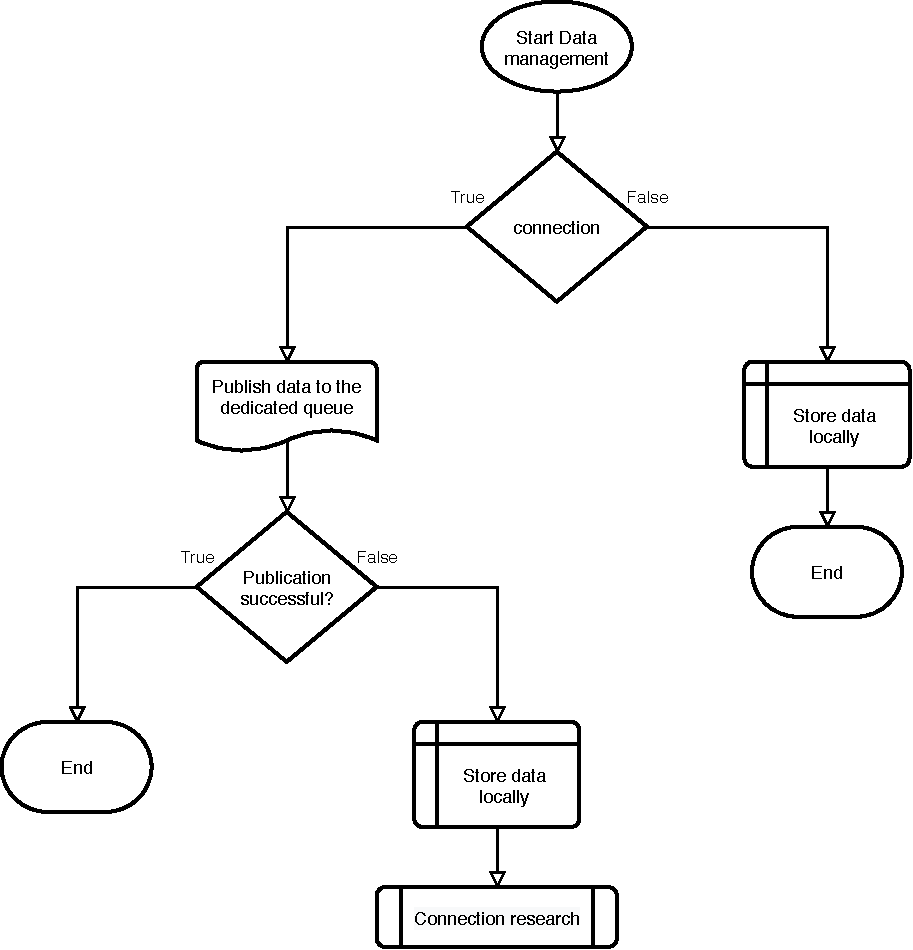
\includegraphics[width=0.5\textwidth]{images/flowdata} 
\caption{Flowchart representing the data management logic.}
\label{fig:flowdata}
\end{figure}

Higher values of the parameters allow us to avoid a continuous transmission of data and to fill the queue on the broker or in the lack of a connection, to open the file to save the data every time a packet is detected. On the other hand, choosing smaller values of the parameters reduces estimation delay, making the system more responsive. In our experiments, we used intermediate values with a maximum number of packets of 50 and a maximum time since the last batch transmission of 60 seconds, which is a good trade-off between congestion and transmission delay.

When the batch is ready, the algorithm for managing what to do with the data starts. If there is no connection, the collected data is stored locally to be sent later when a connection is found.
Instead, if there is a connection with the MQTT broker, the collected data is published to the dedicated queue. If the publication is successful, the flowchart ends. Otherwise, it is stored locally, subsequently the system searches again for a connection.

\begin{figure}[h!]
\begin{minipage}[b]{8.5cm}
\centering
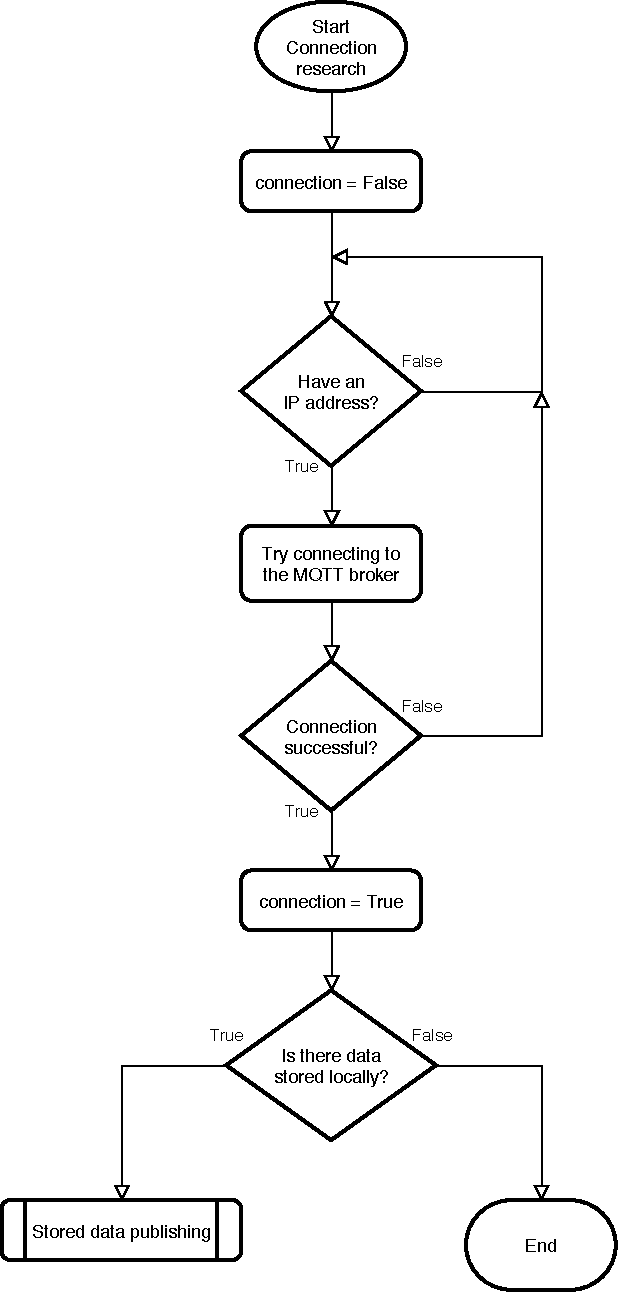
\includegraphics[width=0.75\textwidth]{images/flowconnection}
\caption{Flowchart representing the connection research logic.}
\label{fig:flowconnection}
\end{minipage}
\ \hspace{2mm} \hspace{3mm} \
\begin{minipage}[b]{8.5cm}
\centering
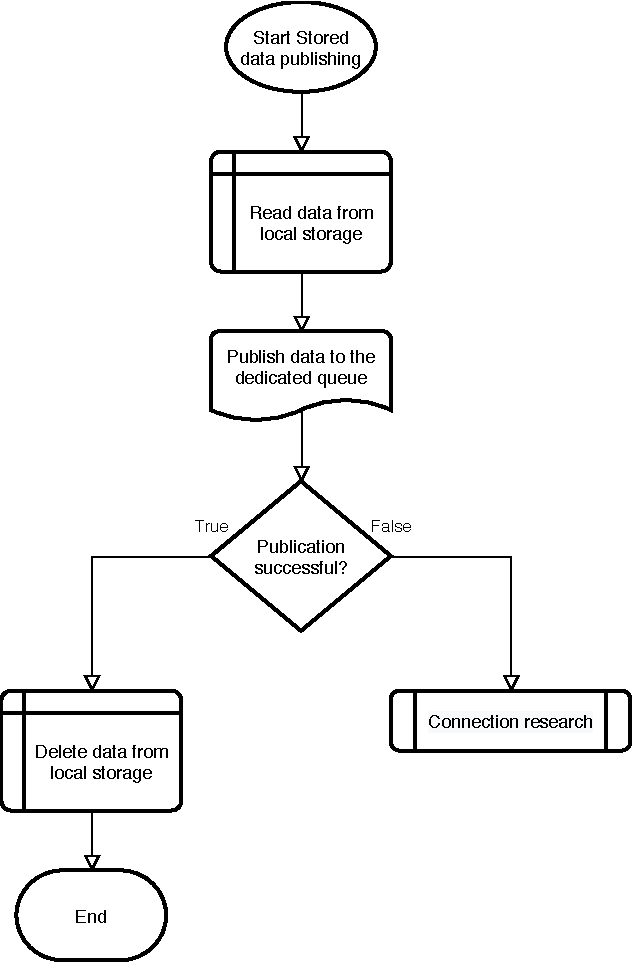
\includegraphics[width=0.75\textwidth]{images/flowstorage}
\caption{Flowchart representing the stored data publishing logic.}
\label{fig:flowstorage}
\end{minipage}
\end{figure}

% \begin{figure}[h]
% \centering 
% 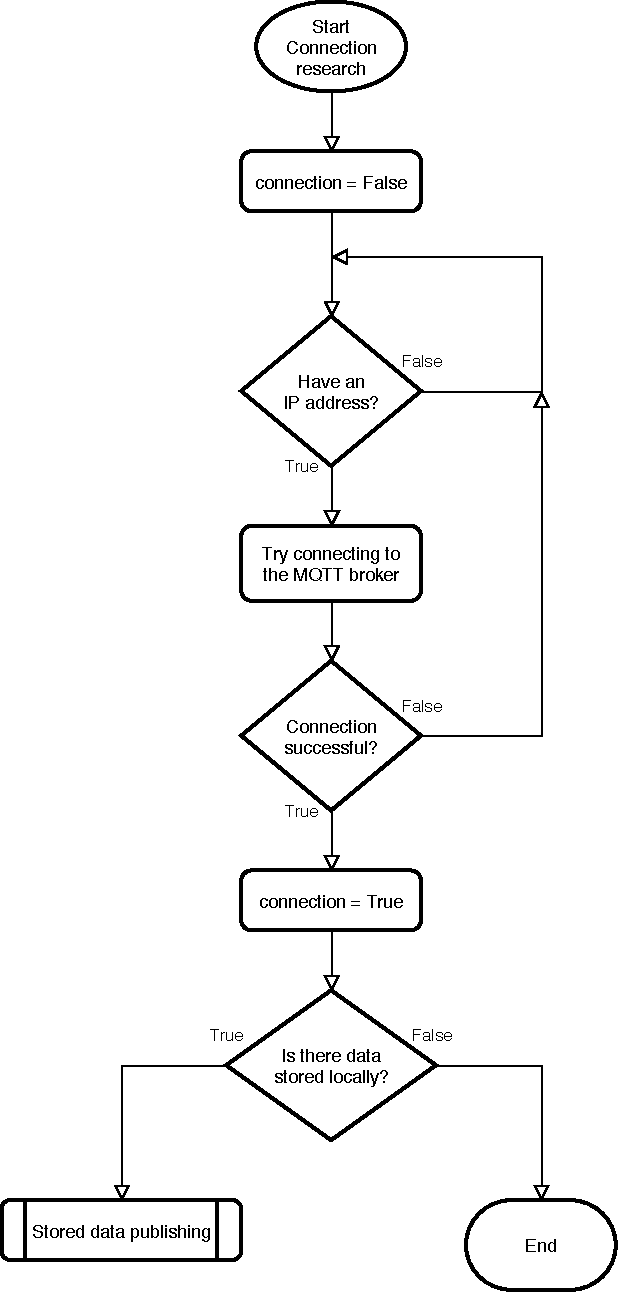
\includegraphics[width=0.5\textwidth]{images/flowconnection} 
% \caption{Flowchart representing the connection research logic.}
% \label{fig:flowconnection}
% \end{figure}

When the data collector is turned on, the system searches also for a connection with the MQTT broker. Figure~\ref{fig:flowconnection} shows the flowchart explaining the logic behind this. Initially, the connection is set = False and the system checks whether the data collector has a peripheral with an IP address for Internet access.
When it has an IP address, a MQTT Client with its credentials tries connecting to the MQTT broker. When the broker is reachable and accepts the client connection, the connection is set = True and if there is data stored locally, it can be published by running the flowchart for the publication of the stored data, shown in figure~\ref{fig:flowstorage}.

% \begin{figure}[h]
% \centering 
% 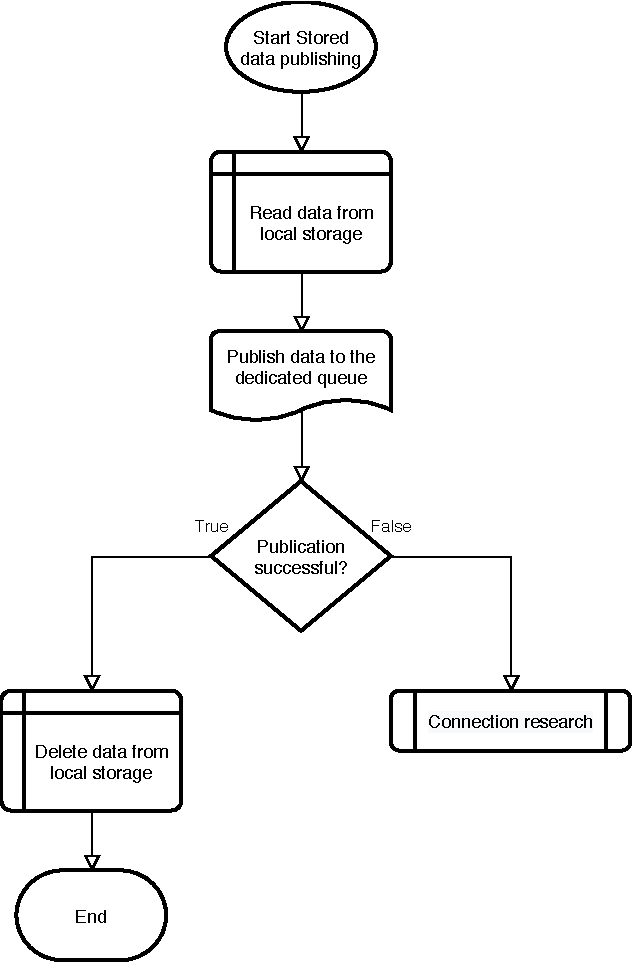
\includegraphics[width=0.5\textwidth]{images/flowstorage} 
% \caption{Flowchart representing the stored data publishing logic.}
% \label{fig:flowstorage}
% \end{figure}

The data is read from the local storage and is published to the dedicated queue. If the publication is successful, the data is deleted from the local storage. Otherwise, it remains stored locally and the system searches again for a connection.


\section{Data forwarding}
\label{sec:forwarding}
\vspace{0.2 cm} 

MQTT\footnote{ website: \url{http://mqtt.org/} } stands for Message Queuing Telemetry Transport. It is a publish/subscribe, extremely simple and lightweight messaging protocol. It is designed to be bandwidth-efficient and to use little battery power. It is efficient in distributing information to one or many receivers. Information is organized in topics. Topics are treated as a hierarchy, using a slash (/) as a separator. These principles make it the ideal protocol for the emerging world of machine-to-machine/Internet of Things and for mobile applications where bandwidth and battery power are limited. It is useful for connections with remote locations, as in our case to send a huge amount of data to the Back-End part. Moreover, it can easily scale from a single device to thousands.

The MQTT protocol defines two types of network entities: a message broker and clients. An MQTT broker is a software running on a computer that receives all messages from the clients and then routes them to the appropriate destination clients. An MQTT client is any device that runs an MQTT library and connects to an MQTT broker over a network.
For security reasons, the MQTT broker can be configured to require clients to use a username and password when connecting. If they match allowed credentials, clients can publish/subscribe to the topics. Otherwise, the connection is refused.
When a publisher has new data to distribute, it publishes this data to the broker. Any client that wants a copy of that message will subscribe to that topic. The broker then distributes the data to any clients that have subscribed to that topic. Multiple clients can receive the message from a single broker. Similarly, multiple publishers can publish topics to a single subscriber.

The protocol uses a publish/subscribe architecture in contrast to HTTP with its request/response paradigm. The main difference to HTTP is that a client does not have to pull the information it needs, but the broker pushes the information to the subscribed client, in case something new has been published. The broker also keeps track of all session information as clients connect and disconnect. If this connection is interrupted by any circumstances, the MQTT broker can buffer all messages and send them to the client when it is back online, setting the clean session bit = False. If clean session bit is true, then all subscriptions will be removed for the client when it disconnects.

Each subscription/publication to the broker can specify a quality of service measure. These are classified in increasing order of overheads:
\begin{itemize}
  \item 0: At most once - the message is sent only once and the publisher and broker take no additional steps to acknowledge delivery to the subscribers (fire and forget, with no confirmation).
  \item 1: At least once - the message is re-tried by the sender (publisher or broker) multiple times until acknowledgment is received (by the broker or the subscribers) (acknowledged delivery).
  \item 2: Exactly once - the sender (publisher or broker) and receiver (broker or the subscribers) engage in a two-level handshake to ensure only one copy of the message is received (assured delivery).
\end{itemize}

For these illustrated features, the MQTT protocol is used in the system for data forwarding. A broker situated on a server, with a static IP address to be accessible and with two dedicated queues is used, one for the collected data, published by the data collector and received by the subscribed Back-End part, and the other one for the Back-End results published by the Back-End and received by the subscribed consumer.
The broker is set up to allow only connections from the data collector, the Back-End and the consumer. They have their own credentials for authentication.

The clean\_session is set = False. If this connection is interrupted by any circumstances, the MQTT broker can buffer all messages and send them to the client when it is back online.
The QoS is set = 2 both in publish and subscribe. To ensure exactly one copy of the data, no loss, no duplicates to clean.


\section{Data cleaning and analysis}
\label{sec:analysis}
\vspace{0.2 cm} 

The Back-End part is situated on a server and receives and stores the collected data. The two main Back-End functionalities are data cleaning and data analysis.

The flowchart representing the data Back-End logic is shown in figure~\ref{fig:flowcleaner}. Initially, the Back-End subscribes to the collected data queue to receive the data when published by the data collector. Input data is managed by adding corollary information for future analysis, e.g. randomization and day of the week. Then this data is stored in a database.

\begin{figure}[h]
\centering 
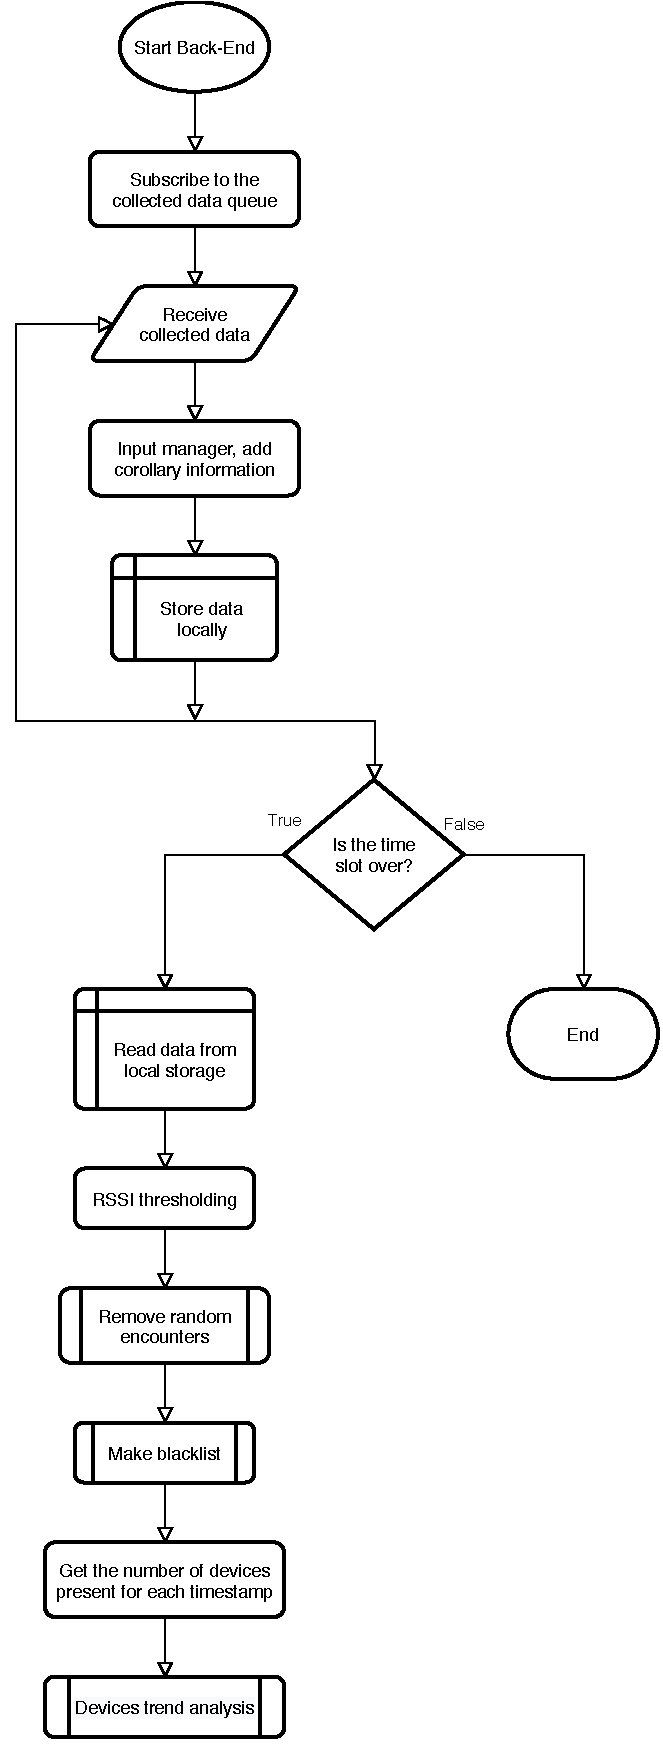
\includegraphics[width=0.35\textwidth]{images/flowcleaner} 
\caption{Flowchart representing the Back-End and the cleaning logic.}
\label{fig:flowcleaner}
\end{figure}

When a time slot is over, the data of the current time slot is read from the database. An RSSI-based threshold is applied to delete data from devices too far from the data collector (to be adapted to the case study, the position of the data collector has to be taken into consideration, as well the environment in which they are located, for cleaning and analysis). Random encounters are removed, as shown in the flowchart in figure~\ref{fig:flowrandom}. Unique devices are extracted with their occurrence timestamps. If there are devices that appear only once or for a short time, they are removed. These parameters have to be adapted to the case study: MIN\_T=20 MIN\_RSSI=-100 (and randomized addresses are removed with this).

% \begin{figure}[h]
% \centering 
% 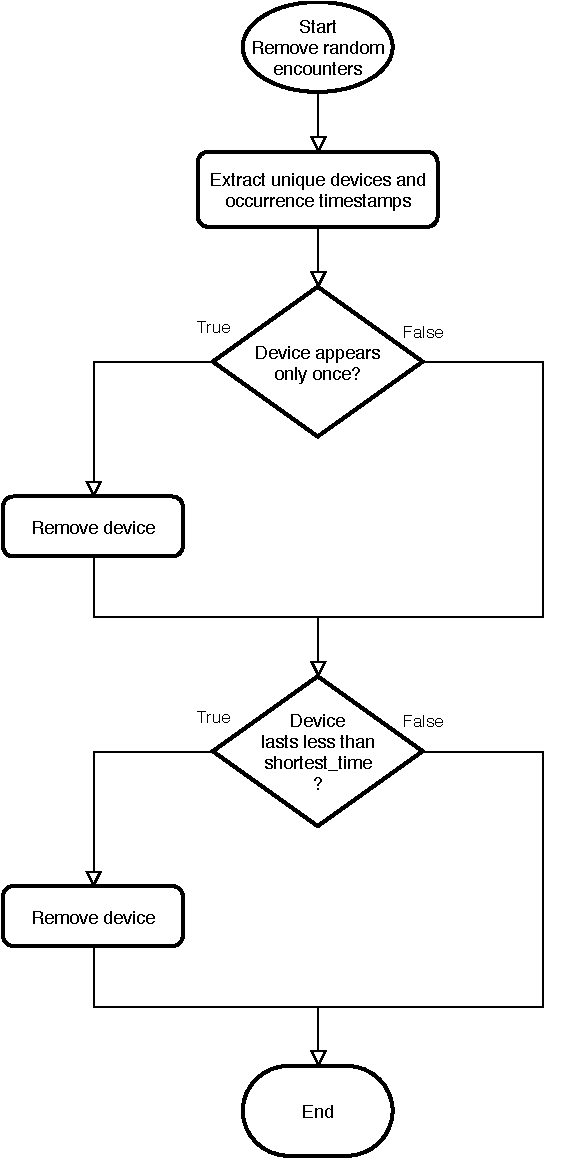
\includegraphics[width=0.5\textwidth]{images/flowrandom} 
% \caption{Flowchart representing the logic of removing casual encounters.}
% \label{fig:flowrandom}
% \end{figure}

Then a blacklist is made to remove the ever-present devices or devices revealed too many times during the day, as shown in the flowchart in figure~\ref{fig:flowblacklist}. A list of occurrences is created with a maximum interrupt time of delta\_t. If there are devices that appears many times or for a long time, they are blacklisted. These parameters have to be adapted to the case study: MAX\_T=7200 MAX\_OCC=10 DELTA\_T=300.
At this point, it is possible to get the number of devices present in the place of interest for each timestamp based on the occurrences of the devices not in the blacklist. The presence of a device is increased by a probe compensation time set as t$_{p}$=15 seconds added before the first Wi-Fi probe request detection of the MAC address and after the last one. This is done to consider the time that passes between the actual presence of the device and the actual transmission of the first Wi-Fi probe request.

% \begin{figure}[h]
% \centering 
% 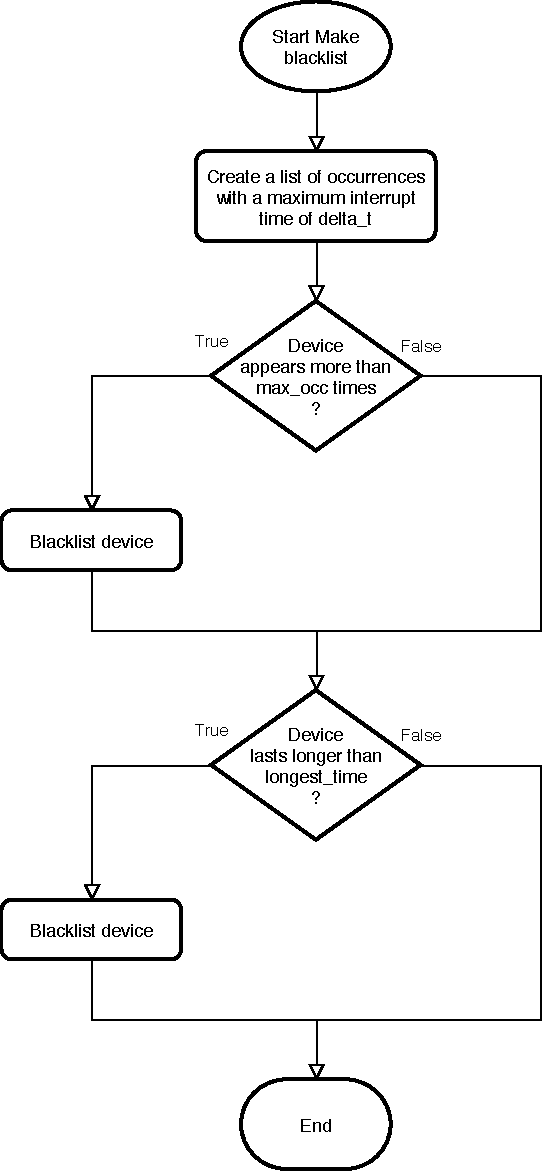
\includegraphics[width=0.5\textwidth]{images/flowblacklist} 
% \caption{Flowchart representing the logic of making the blacklist.}
% \label{fig:flowblacklist}
% \end{figure}

\begin{figure}
\begin{minipage}[b]{8.5cm}
\centering
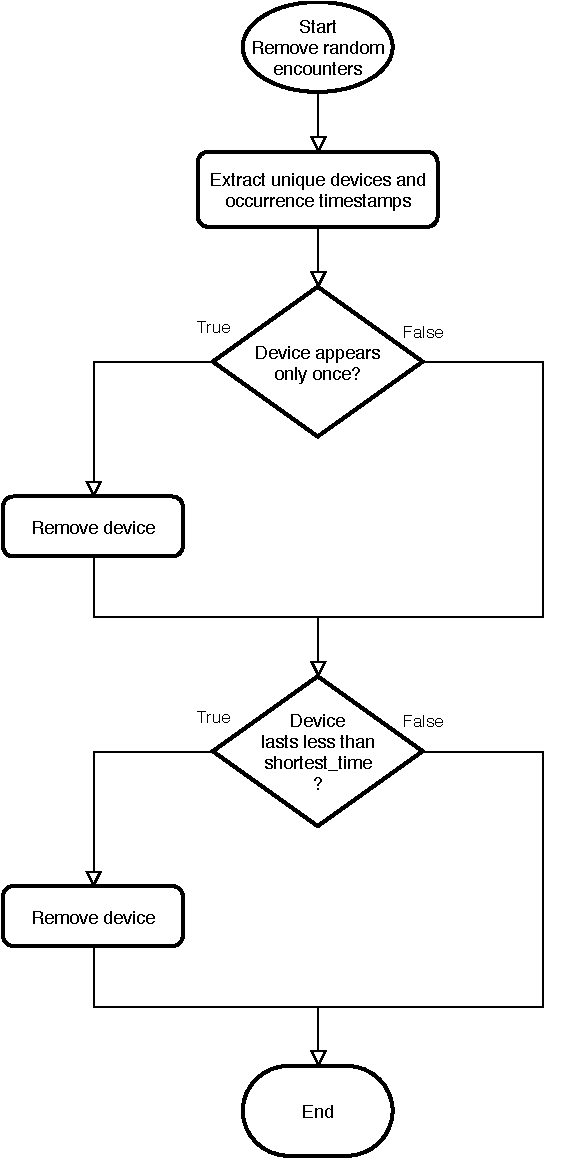
\includegraphics[width=0.55\textwidth]{images/flowrandom}
\caption{Flowchart representing the logic of removing random encounters.}
\label{fig:flowrandom}
\end{minipage}
\ \hspace{2mm} \hspace{3mm} \
\begin{minipage}[b]{8.5cm}
\centering
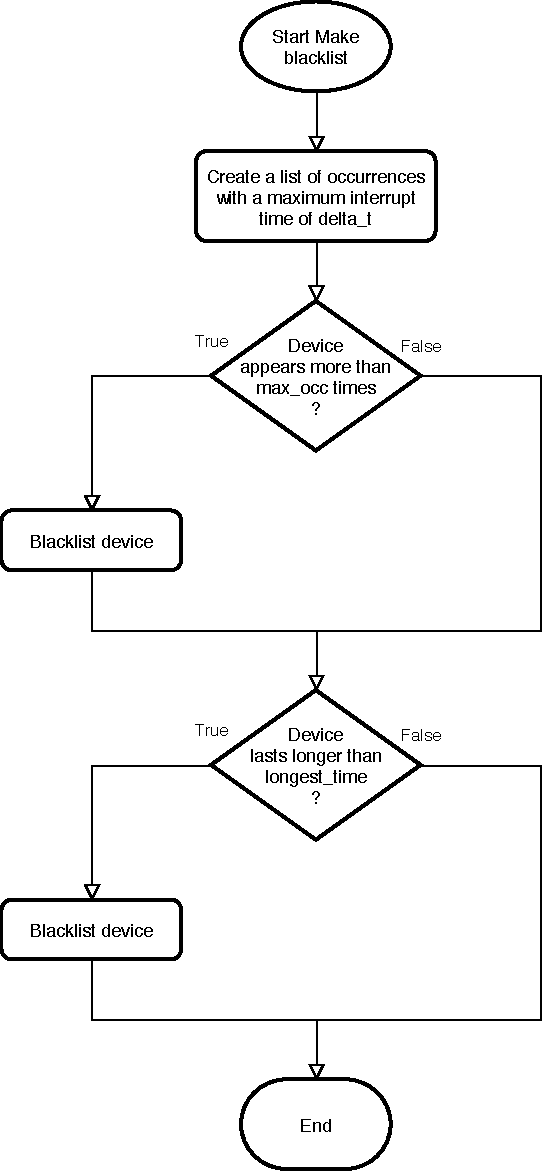
\includegraphics[width=0.55\textwidth]{images/flowblacklist}
\caption{Flowchart representing the logic of making the blacklist.}
\label{fig:flowblacklist}
\end{minipage}
\end{figure}

Finally, data analysis is performed, as shown in the flowchart in figure~\ref{fig:flowML}. Trend (raising/lowering) and seasonality (repetition of the components) of the number of devices are extracted using a decomposition of the corresponding temporal series. Once these two variables are known, it is possible to apply to them the correct polynomial approximation relating to the current time slot to get the estimation of the number of people present in the place of interest.

% \begin{figure}[h]
% \centering 
% 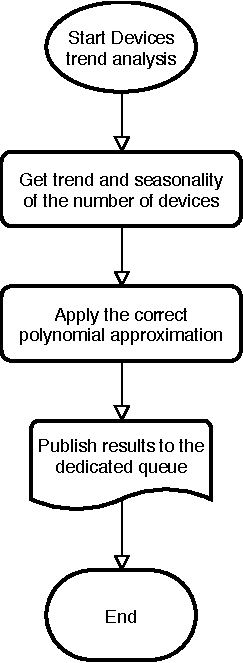
\includegraphics[width=0.3\textwidth]{images/flowML} 
% \caption{Flowchart representing the data analysis logic.}
% \label{fig:flowML}
% \end{figure}

% \begin{figure}[h]
% \centering 
% 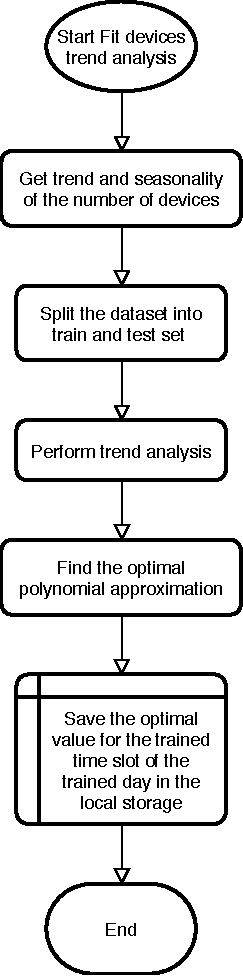
\includegraphics[width=0.3\textwidth]{images/flowtrainML} 
% \caption{Flowchart representing the ML training logic.}
% \label{fig:flowtrainML}
% \end{figure}

\begin{figure}
\begin{minipage}[b]{8.5cm}
\centering
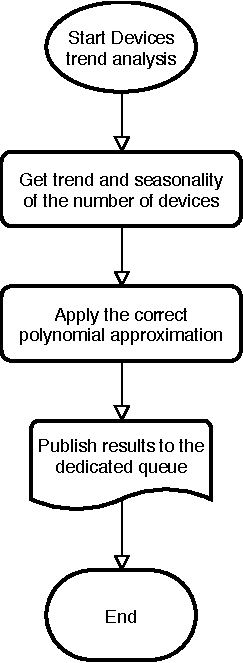
\includegraphics[width=0.3\textwidth]{images/flowML}
\caption{Flowchart representing the data analysis logic.}
\label{fig:flowML}
\end{minipage}
\ \hspace{2mm} \hspace{3mm} \
\begin{minipage}[b]{8.5cm}
\centering
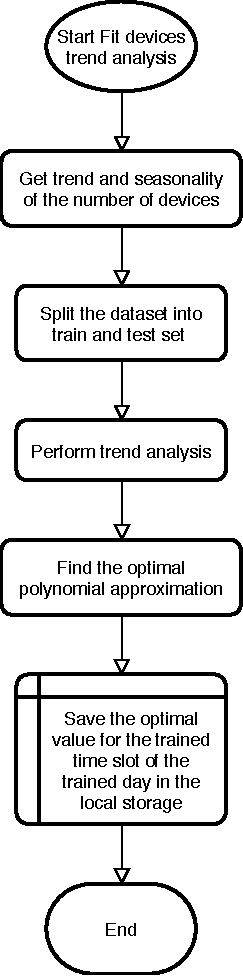
\includegraphics[width=0.3\textwidth]{images/flowtrainML}
\caption{Flowchart representing the ML training logic.}
\label{fig:flowtrainML}
\end{minipage}
\end{figure}

I did not develop the part of machine learning, but I integrated an existing one into this project to get the final results, i.e. the number of people in the place of interest for each timestamp. Then the results, when available, are published to the dedicated queue (Back-End results) to be received by the subscribed consumer who could use this information to improve his business.


\vspace{0.1 cm}
\subsection{Preparation of the model}
\label{sec:model}
\vspace{0.1 cm} 

The best degree and coefficients of the polynomial approximation are calculated during the preparation of the model that consist in a training phase for each time slot of each day of the week, using manually-collected ground truth. Figure~\ref{fig:flowtrainML} shows the flowchart of the logic used in that phase.

In the timestamps where the ground truth is collected by the number of devices revealed in these timestamps, we get the trend and the seasonality of the annotated dataset.
Using this dataset we train a regressor to find the best polynomial approximation for each considered time slot. We initially divide the dataset into train set and test set. The machine learning model performs a trend analysis to find the best polynomial approximation for each time slot. These values of the coefficients are stored to be used in the different time slots when data are collected to get the correct estimate of the number of people.


\vspace{0.1 cm}
\subsection{Management of time processes}
\label{sec:model}
\vspace{0.1 cm} 

There are 3 main time processes to manage:
\begin{itemize}
  \item Probe revelations from the data collector: a random point process with different MAC addresses.
  \item Presence of devices: a cadlag step function based on the revelations of the MAC addresses, obtained after the cleaning of the collected data. Figure~\ref{fig:presenceMAC} show how the presence of the devices is obtained. For example, presence MAC$_1$ $= 1 \cdot \chi_{[ t_{0} - t_{p}, t_{3} + t_{p} )} + 1 \cdot \chi_{[ t_{6} - t_{p}, t_{9} + t_{p} )}$. So by summing the presence of the different MAC addresses, the presence of devices is obtained: Presence of devices $= \sum_i$ presence MAC$_i$.
  \item Collection of the ground truth: a sampling of the number people present, a random point process asynchronous with respect to the probe revealed and devices revealed. Figure~\ref{fig:GTprocess} shows how the ground truth is collected. Dirac delta function represent the sampling of the number of people presence: GT(t$_i$) $= g(t) \cdot \delta(t - t_{i})$
\end{itemize}

\begin{figure}[h]
\centering 
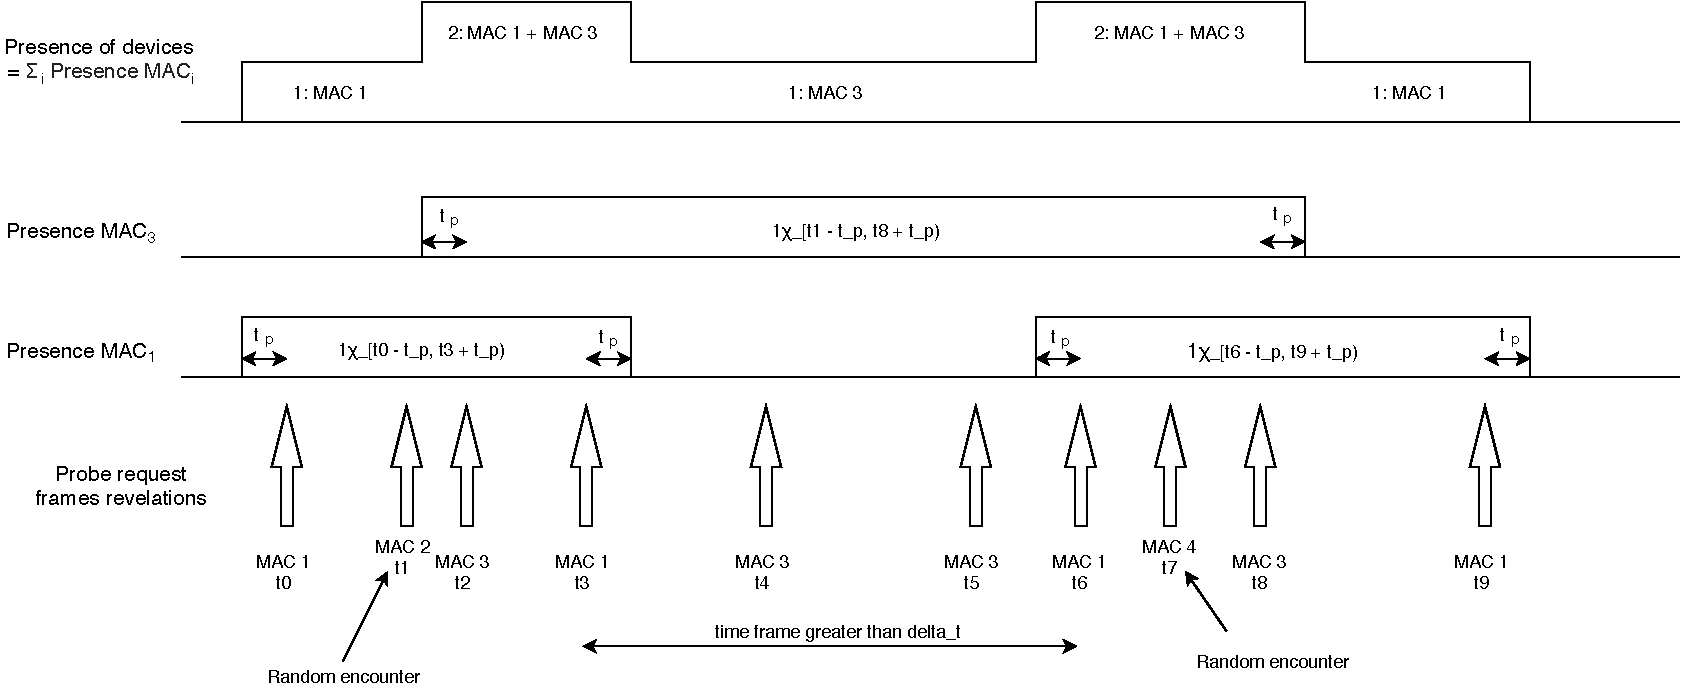
\includegraphics[width=0.8\textwidth]{images/presenceMAC} 
\caption{Illustration of how the presence of devices is calculated.}
\label{fig:presenceMAC}
\end{figure}

\begin{figure}[h]
\centering 
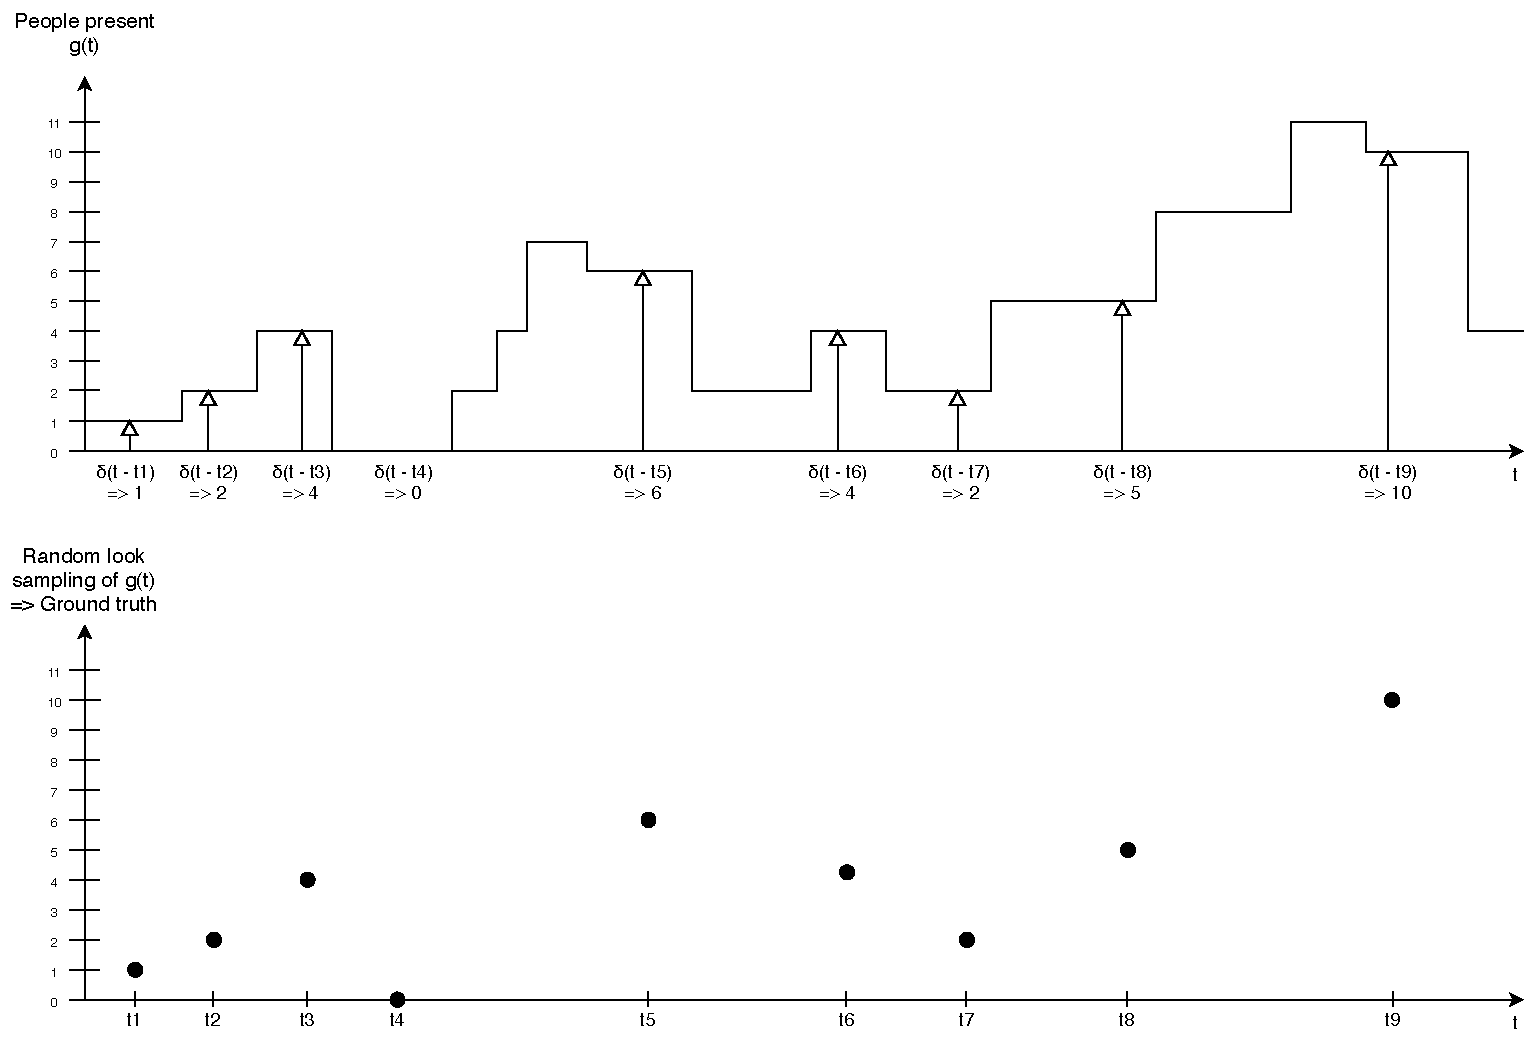
\includegraphics[width=0.65\textwidth]{images/GTprocess} 
\caption{Illustration of the collection of the ground truth.}
\label{fig:GTprocess}
\end{figure}

      \afterpage{\null\thispagestyle{empty}\clearpage}
      \chapter{Implementation}
\label{cha:implementation}
\vspace{0.4 cm} 

This chapter presents how the components of the system have been implemented.
Starting by describing the implementation of the data collector on a Raspberry Pi and then explaining how the Mosquitto MQTT Broker, the MongoDB database and the two Back-End parts, one for receiving and storing the data and the other one for analyzing the data, has been implemented using Docker containers. After this chapter, it will be clear how the system was implemented for the testing and validation, that are discussed in the next chapter.


\section{Data collector implementation}
\label{sec:collector}
\vspace{0.2 cm} 

The data collector is implemented on a Raspberry Pi model 2B using:
\begin{itemize}
  \item A EDUP 802.11n Wi-Fi Dongle (Range $\sim$ 10 meters) is used with the Scapy library for Wi-Fi packets sniffing and information extraction.
  \item A Real Time Clock Module is used for timestamp detection.
  \item From hashlib Python module BLAKE2s, an implementation of the BLAKE2, is used for MAC address anonymization.
  \item JSON Python module is used to store data locally and to read and publish them later.
  \item Another EDUP 802.11n Wi-Fi Dongle (Range $\sim$ 10 meters) is used with the Netifaces library for managing the connection.
  \item Paho-MQTT library is used for running the MQTT client and the data forwarding.\\publish(``topic'', payload=json.dumps(data), qos=2)
\end{itemize}

% Client(client\_id=``name'', clean\_session=False), connect(``broker\_address'', port=1883)

% username\_pw\_set(``username'', password=``password'')

% publish(``topic'', payload=json.dumps(data), qos=2)

% subscribe(``topic'', qos=2)


\section{Tool for ground truth management}
\label{sec:toolgt}
\vspace{0.2 cm} 

I developed two scripts to manage the ground truth. One for collecting the ground truth and made the annotations in the place of interest. When the number of people present is written on the input of the program, it saves this information with the timestamp, the day of the week on a file.
The other script is used to load the collected ground truth in the MongoDB using PyMongo MongoClient for accessing the database and storing data.


\section{Cloud infrastructure implementation}
\label{sec:cloudinfrastructure}
\vspace{0.2 cm} 

On the U-hopper cloud infrastructure there are the other components running in Docker Containers:
\begin{itemize}
  \item As MQTT broker we used Eclipse Mosquitto\footnote{ website: \url{https://hub.docker.com/_/eclipse-mosquitto} }, an open-source MQTT broker.
  \item As database we used MongoDB\footnote{ website: \url{https://hub.docker.com/_/mongo} } for its simplicity in handling JSON files.
  \item For running the receiver MQTT client we used the Paho-MQTT library for receiving the data.\\subscribe(``topic'', qos=2)
  \item For running the MongoClient we used the PyMongo library to access the MongoDB and store the data.
  \item In the analyzer, we used PyMongo library and Pandas library to read and manage the data stored in MongoDB with a MongoClient to get the data and a Pandas DataFrame to clean the data and get the number of devices.
  \item Sklearn library is used to analyze the cleaned data and train the regressor using the ground truth. This library is used to implement the machine learning part.
\end{itemize}

Finally, I developed a script to calculate the metrics, e.g. error information, and compute the graphs, e.g. histograms, error distribution and comparison of detected devices and of people estimated with the real number of people present.

      \afterpage{\null\thispagestyle{empty}\clearpage}
      \chapter{Evaluation}
\label{cha:evaluation}
\vspace{0.5 cm} 

Write about the implementation \dots

\vspace{0.5 cm} 
\section{Experimental validation}
\label{sec:expval}
\vspace{0.5 cm} 

Write about the experiments \dots


\vspace{0.5 cm} 
\section{Evaluation of the results}
\label{sec:evalres}
\vspace{0.5 cm} 

Write an evaluation \dots

      \afterpage{\null\thispagestyle{empty}\clearpage}
      \chapter{Conclusions}
\label{cha:conclusions}
\vspace{0.5 cm} 

The work is done \dots

\vspace{0.5 cm} 
\section{Future work}
\label{sec:future}
\vspace{0.5 cm} 

Write about future work \dots

      \afterpage{\null\thispagestyle{empty}\clearpage}
      
    \endgroup


    % bibliografia in formato bibtex
    %
    % aggiunta del capitolo nell'indice
    \addcontentsline{toc}{chapter}{Bibliography}
    % stile con ordinamento alfabetico in funzione degli autori
    \bibliographystyle{plain}
    \bibliography{bibliography}
%%%%%%%%%%%%%%%%%%%%%%%%%%%%%%%%%%%%%%%%%%%%%%%%%%%%%%%%%%%%%%%%%%%%%%%%%%
%%%%%%%%%%%%%%%%%%%%%%%%%%%%%%%%%%%%%%%%%%%%%%%%%%%%%%%%%%%%%%%%%%%%%%%%%%
%% Nota
%%%%%%%%%%%%%%%%%%%%%%%%%%%%%%%%%%%%%%%%%%%%%%%%%%%%%%%%%%%%%%%%%%%%%%%%%%
%% Nella bibliografia devono essere riportati tutte le fonti consultate 
%% per lo svolgimento della tesi. La bibliografia deve essere redatta 
%% in ordine alfabetico sul cognome del primo autore. 
%% 
%% La forma della citazione bibliografica va inserita secondo la fonte utilizzata:
%% 
%% LIBRI
%% Cognome e iniziale del nome autore/autori, la data di edizione, titolo, casa editrice, eventuale numero dell’edizione. 
%% 
%% ARTICOLI DI RIVISTA
%% Cognome e iniziale del nome autore/autori, titolo articolo, titolo rivista, volume, numero, numero di pagine.
%% 
%% ARTICOLI DI CONFERENZA
%% Cognome e iniziale del nome autore/autori (anno), titolo articolo, titolo conferenza, luogo della conferenza (città e paese), date della conferenza, numero di pagine. 
%% 
%% SITOGRAFIA
%% La sitografia contiene un elenco di indirizzi Web consultati e disposti in ordine alfabetico. 
%% E’ necessario:
%%   Copiare la URL (l’indirizzo web) specifica della pagina consultata
%%   Se disponibile, indicare il cognome e nome dell’autore, il titolo ed eventuale sottotitolo del testo
%%   Se disponibile, inserire la data di ultima consultazione della risorsa (gg/mm/aaaa).    
%%%%%%%%%%%%%%%%%%%%%%%%%%%%%%%%%%%%%%%%%%%%%%%%%%%%%%%%%%%%%%%%%%%%%%%%%%
%%%%%%%%%%%%%%%%%%%%%%%%%%%%%%%%%%%%%%%%%%%%%%%%%%%%%%%%%%%%%%%%%%%%%%%%%%
    

    %titleformat{\chapter}
    %    {\normalfont\Huge\bfseries}{Attachment \thechapter}{1em}{}
    % sezione Allegati - opzionale
    %\appendix
    %\chapter{Title of the first attachment}
\vspace{0.4 cm} 

The first attachment


\section{Title}
\vspace{0.2 cm} 
The title of the first attachment


\subsection{Subtitle}
\vspace{0.2 cm} 
The subtitle of the first attachment


\chapter{Title of the second attachment}
\vspace{0.2 cm} 

The second attachment


\section{Title}
\vspace{0.2 cm} 
The title of the second attachment


\subsection{Subtitle}
\vspace{0.2 cm} 
The subtitle of the second attachment


\end{document}
